\subsection{Обратная связь по выходу}
\selectlanguage{russian}

\begin{figure}[bt]
	\centering
	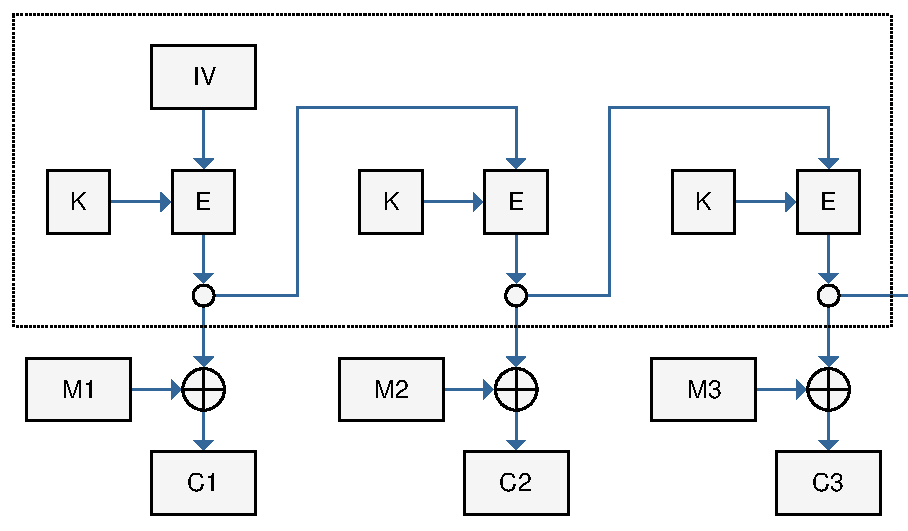
\includegraphics[width=1\textwidth]{pic/OFB}
	\caption{Режим обратной связи по выходу. Пунктирной рамкой выделена область формирования \emph{гаммы}, независящей от открытого текста.}
	\label{fig:OFB}
\end{figure}

В предыдущих режимах входными блоками для функции шифрования были непосредственно блоки открытого текста. В режиме обратной связи по выходу (\langen{Output Feedback, OFB}, рис.~\ref{fig:OFB}) блоки открытого текста непосредственно на вход функции шифрования не поступают. Вместо этого функция шифрования генерирует псевдослучайный поток байтов, который суммируется побитово по модулю $2$ с открытым текстом для получения шифртекста. Шифрование осуществляют по правилу:
\[ \begin{array}{l}
    K_0 = \textrm{IV}, \\
    K_j = E_K(K_{j-1}), ~ j = 1, 2, \dots, n, \\
    C_j = K_j \oplus M_j.
\end{array} \]

Здесь текущий ключ $K_j$ есть результат шифрования предыдущего ключа $K_{j-1}$. Начальное значение $K_0$ известно криптографу и легальному пользователю. На приёмной стороне расшифрование выполняют по правилу:
\[ \begin{array}{l}
    K_0 = \textrm{IV}, \\
    K_j = E_K(K_{j-1}), ~ j = 1, 2, \dots, n, \\
    M_j = K_j \oplus C_j.
\end{array} \]

Как и в режиме CBC, вектор инициализации $\textrm{IV}$ может быть выбран случайно и передан вместе с шифрованным текстом, либо вычислен на основе одноразовых меток. Здесь особенно важна уникальность вектора инициализации.

Достоинство этого режима состоит в полном совпадении операций шифрования и расшифрования. Кроме того, в этом режиме не надо проводить операцию дополнения открытого текста.
